%!TEX root = ../dokumentation.tex

\chapter{Kommunikation zwischen Bilderkennung und Roboter\footnote{besseren Namen einfallen lassen, der dem neuen Inhalt gerecht wird(Kommunikation und Umrechnung oder so}}
\label{cha:Kommunikation zwischen Bilderkennung und Roboter}
\section{Kommunikation}
Die Kommunikation zwischen dem Roboter und dem Airhockeyprogramm erfolgt über das Ethernet. Dabei haben wir uns für die Kommunikation über Sockets entschieden, da dies die gängigste Methode ist und sowohl von der Programmiersprache des Roboters als auch von Python beherrscht wird. Der Roboter fungiert dabei als Client der sich mit einem Server verbindet. Die PC mit der Roboter-KI ist in diesem Fall der Server. Es hat keinen besonderen Grund wieso wir das so rum getan haben. Dies kann genauso gut auch andersrum implementiert werden, also mit dem Roboter als Server und dem PC-Programm als Client. Wir hatten beide Variante ausgetestet und mehrfach zwischen beiden hin- und hergewechselt. Da wir aber bei unseren Tests keine Geschwindigkeitsunterschiede zwischen beiden feststellen konnten, haben wir dann letztenendes die oben genannte Variante einfach gelassen.

Mithilfe von Sockets wird eine Folge von Bytes übertragen. Da sowohl erweiterter ANSI-Code als auch UTF-8 ein Byte groß sind, könnte man diese Folge von Bytes auch als eine Folge von Zeichen interpretieren. Wie dies die jeweilige Programmiersprache interpretiert sollte man am besten im jeweiligen Handbuch nachlesen. In unseren Fall hat RAPID und Python 2.7 die übertragenen Daten als String angesehen, also als eine Folge von Zeichen. 
%Dies war recht gelegen, da dadurch keine komplizeirten Umformungen vorgenommen werden mussten. 
Übertragen wurde nur die Position, zu der sich der Roboter bewegen soll.  Da sich das Spielfeld nur auf einer 2-Dimensionalen Ebene befindet, waren dazu nur eine X- und Y-Koordinate nötig. Diese wurden durch ein Semikolon getrennt, wodurch die Daten wieder recht einfach auf Seite des Roboters getrennt werden konnten. Anfänglich war das nur eine Kommunikation in eine Richtung, wurde aber später noch ergänzt um eine Art \enquote{Bereit}, das vom Roboter zurück gesendet wurde, sobald dieser seine Position erreicht hat und neue Befehle entgegennehmen kann. 

\section{Erweiterung des Bilderkennungsprogramms um Kommunikationsmodul}
Die Kommunikation zwischen PC und Roboter erfolgt wie in Kapitel \ref{cha:Kommunikation zwischen Bilderkennung und Roboter} auf Seite \pageref{cha:Kommunikation zwischen Bilderkennung und Roboter} beschrieben mithilfe von Sockets. Der PC öffnet einen Serversocket und der Roboter einen Clientsocket. Die Socketkommunikation funktioniert nach dem TCP/IP Verfahren. Man weiß also immer ob die Kommunikation zu Stande kam.
Ursprünglich hatten wir für jede Übertragung einen neuen Socket erstellt, die Daten übermittelt und anschließend den Socket wieder geschlossen. Dies haben wir so praktiziert da in der Python Dokumentation geschrieben stand, das Sockets normalerweise nur für eine Übertratung oder eine kleine Folge von Übertragungen genutzt werden und anschließend wieder geschlossen werden.
\begin{quote}
When the connect completes, the socket s can be used to send in a request for the text of the page. The same socket will read the reply, and then be destroyed. That’s right, destroyed. Client sockets are normally only used for one exchange (or a small set of sequential exchanges).\cite{Python-Doku}
\end{quote}
Da auch der Socket auf der Serverseite wieder freigegeben werden musste, konnte bei einem erneuten Kommunikationsversuches des Clients keine Verbindung zum Serversocket des Roboters hergestellt werden. Dadurch wussten wir auch automatisch, dass der Roboter sich noch bewegt und keine neuen Befehle entgegen nehmen kann. Wir hatten für die Sockets eine timeoutzeit von 1/100s eingestellt. Somit hat ein Kommunikationsversuch mit dem Roboter maximal 1/50s benötigt. Einmal  1/100s für die Verbindung aufbauen und einmal 1/100s für die Daten senden. Da wir mit der angebauten 30 FPS Kamera nur alle 1/30s neue Bilder erhielten, mit denen man neu rechnen muss, war diese 1/50s Maximalzeit auch ausreichend. Es hat sich aber herausgestellt, das anscheinend durch das Socket öffnen und schließen eine viel größere Zeit benötigt wird. Denn zwischen dem senden eines Befehls und dem erneuten senden eines Befehls vergingen mindestens eine halbe Sekunde, selbst wenn sich der Roboter gar nicht bewegen muss. Hinzu kam noch, dass das Schließen des Sockets auf Serverseite länger benötigt als auf Clientseite. Die Zeit die zum Schließen des Serversockets benötigt wurde, hat wahrscheinlich auch diese halbe Sekunde Latenzzeit verursacht. Es entstand aber auch noch ein anderer Nebeneffekt dadurch. Denn der Clientsocket hat in dieser Zeit immer noch eine Verbindung mit dem Serversocket erstellen können und hat somit auch noch Daten geschickt. Diese Daten kamen aber nicht mehr beim Serversocket an, sondern wurden irgendwo zwischen gebuffert. Beim nächsten öffnen des Serversockets wurden dann diese Daten sofort empfangen und verarbeitet. Durch diesen Buffer entstanden immer Ausreißer des Roboters, die wir uns lange Zeit nicht erklären konnten. Wir haben dieses Problem dann erst mitbekommen, nachdem wir ein paar Tests durchgeführt haben um die Geschwindigkeit des Roboters festzustellen. Das Programm für die Test hat dann häufig bis zu 3 Werte hintereinander geschickt, bevor es gewartet hat, das der Roboter einen neuen Serversocket geöffnet hat. 

\begin{wrapfigure}{R}{0pt}
	\vspace{-15pt}
	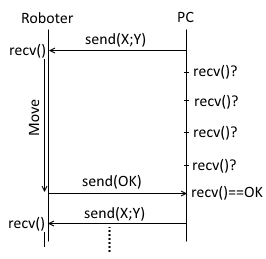
\includegraphics{Socketkommunikation.png}
	\vspace{-15pt}
	\caption{ Veranschaulichung der Socketkommunikation}
	\vspace{-15pt}
	\label{img:Socketkommunikation}
\end{wrapfigure}
Wir führten darauf hin einen Two-Way-Handshake ein. Nach dem der Roboter seine Zielposition erreicht hat, hat dieser ein OK zurückgeschickt.Ursprünglich hatten wir dann solange gewartet bis der Roboter sein OK geschickt hat. Dabei hatten wir nur eins nicht beachtet und zwar dass das Programm sequenziell abläuft und während der Wartezeit wie eingefroren ist. Das heißt wir haben dann auch nur alle halbe Sekunde das neue Bild von der Kamera ausgewertet. Dadurch konnte das ganze Programm nicht mehr ordentlich reagieren, da keine vernünftigen Puckbewegungen mehr errechnet werden konnten. Beim zweiten Versuch, wurde pro Programmzyklus nur einmal überprüft ob der Roboter sein OK gesendet hat. Wenn dieses OK nicht kam wurde auf das neue Bild gewartet und dann erneut abgefragt bis der Roboter sein OK gesendet hat. Dies wird im Bild \ref{img:Socketkommunikation} auf Seite \pageref{img:Socketkommunikation} nochmal grafisch zur besseren Verständlichkeit dargestellt. Dadurch konnten wir zwar die Aussreißer stark reduzieren, aber es gab immer noch die hohe Latenzzeit von mindestens einer halben Sekunde. Am Ende haben wir uns dann gegen die Empfehlung der Python Dokumentation entschieden und nur am Amfang des Programmstartes einen Socket zu öffnen und diesen über die komplette Programmlaufzeit offen zu lassen. Wir konnten auch bei längeren Laufzeiten von einer halben Stunde und mehr keine Irregularitäten feststellen, weshalb wir entschieden haben, dies so zu belassen. Der einzige Nachteil war, dass wir die Sockets auf diese Art und Weise nicht ordentlich schließen konnten, denn es gibt in Python keinen Deconstructor, wie man ihn aus anderen Objektorientierten Programmiersprachen kennt. Deshalb muss man nach Abbruch des Programms 1-2 Minuten warten bis das Betriebssystem den Socket von alleine wieder schließt. Leider kann man ohne eine Referenz auf den Socket diesen nicht manuell schließen. Und da wir nicht jedesmal den Programmcode umschreiben wollten um einen neuen Port einzutragen, mussten wir zwischen den Tests immer ein weilchen warten.


\section{Umrechnung vom Bildkoordinatensystem und Roboterkoordinatensystem}

\begin{wrapfigure}{R}{0pt}
	\vspace{-15pt}
	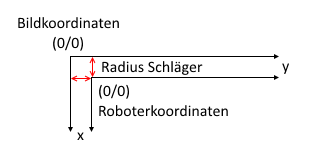
\includegraphics{Umrechnung_Koordinatensysteme.png}
	\vspace{-15pt}
	\caption{ Veranschaulichung der Koordinatensystemunterschiede}
	\vspace{-15pt}
	\label{img:Umrechnung Koordinatensysteme}
\end{wrapfigure}

Bilderkennung und Roboter nutzen unterschiedliche Koordinatensysteme. Das Bildkoordinatensystem enthält für X und Y Werte von 0 bis 1. Dieses geht von einer Ecke (0/0) bis in die entgegengesetzte Ecke (1/1). Es verwendet ein normalisiertes Koordinatensystem. Somit ist es abhängig, wie die Kamera auf das Spielfeld zeigt. Der Abstand zwischen 2 Punkten ist somit mit unterschiedlichen Kameraeinstellungen auch unterschiedlich. Das Roboterkoordinatensystem verwendet stattdessen mm für ihre Koordinaten. Ein Punkt (0/0) ist somit immer 10mm vom Punkt (10/0) entfernt. Hinzu kommt aber noch, das das Roboterkoordinatensystem einen kleinen Offset vom Bildkoordinatensystem hat. Der Punkt (0/0) im Roboterkoordinatensystem ist ein anderer Punkt im Bildkoordinatensystem. Das liegt daran, dass der Schläger einen gewissen Durchmesser hat und somit nicht exakt in die Ecke gefahren werden kann bei der Kalibrierung. Diesen Unterschied kann man auch gut in der Grafik \ref{img:Umrechnung Koordinatensysteme} auf der Seite \pageref{img:Umrechnung Koordinatensysteme} erkennen. Für die Umrechung haben wir folgende Gleichungen aufgestellt:

$
\begin{array}{c}
x_{Roboter} = (x_{Bild} * Tischtiefe) - Durchmesser Schlaeger / 2.0 + x_{Bild} * durchmesserSchlaeger \\
y_{Roboter} = (y_{Bild} * Tischbreite) - Durchmesser Schlaeger / 2.0 + y_{Bild} * durchmesserSchlaeger
\end{array}
$

Nur in einem Fall nutzen wir die Rücktransformation für die Y"~Koordinate. Dafür wurde die Gleichung folgendermaßen umgestellt:

$y_{Bild} = (y_{Rob} + durchmesserSchlaeger / 2.0) / (Tischbreite +  durchmesserSchlaeger)$ 